\documentclass{beamer}
\usepackage[dvipsnames]{xcolor}
\usepackage{listings}
\usepackage[most]{tcolorbox}
\usepackage{hyperref}
\usepackage{tikz}
\usepackage{graphicx}

\newcommand\YAMLcolonstyle{\color{red}\mdseries}
\newcommand\YAMLkeystyle{\color{black}\bfseries}
\newcommand\YAMLvaluestyle{\color{blue}\mdseries}
\definecolor{gray75}{gray}{0.75}
\definecolor{codegreen}{rgb}{0,0.6,0}
\definecolor{codegray}{rgb}{0.5,0.5,0.5}
\definecolor{codepurple}{rgb}{0.58,0,0.82}
\definecolor{backcolour}{rgb}{0.95,0.95,0.92}
\definecolor{mygray}{RGB}{240,240,240}


\newcommand*{\ClipSep}{0.4cm}%

\makeatletter

% here is a macro expanding to the name of the language
% (handy if you decide to change it further down the road)
\newcommand\language@yaml{yaml}

\expandafter\expandafter\expandafter\lstdefinelanguage
\expandafter{\language@yaml}
{
  keywords={true,false,null,y,n},
  keywordstyle=\color{darkgray}\bfseries,
  basicstyle=\YAMLkeystyle,                                 % assuming a key comes first
  sensitive=false,
  comment=[l]{\#},
  morecomment=[s]{/*}{*/},
  commentstyle=\color{purple}\ttfamily,
  stringstyle=\YAMLvaluestyle\ttfamily,
  moredelim=[l][\color{orange}]{\&},
  moredelim=[l][\color{magenta}]{*},
  moredelim=**[il][\YAMLcolonstyle{:}\YAMLvaluestyle]{:},   % switch to value style at :
  morestring=[b]',
  morestring=[b]",
  literate =    {---}{{\ProcessThreeDashes}}3
                {>}{{\textcolor{red}\textgreater}}1     
                {|}{{\textcolor{red}\textbar}}1 
                {\ -\ }{{\mdseries\ -\ }}3,
}

% switch to key style at EOL
\lst@AddToHook{EveryLine}{\ifx\lst@language\language@yaml\YAMLkeystyle\fi}
\makeatother

\lstdefinestyle{customyaml}{
    backgroundcolor=\color{backcolour},
    commentstyle=\color{codegreen},
    keywordstyle=\color{magenta},
    numberstyle=\tiny\color{codegray},
    stringstyle=\color{codepurple},
    basicstyle=\ttfamily\footnotesize,
    breakatwhitespace=false,
    breaklines=true,
    captionpos=b,
    keepspaces=true,
    numbers=left,
    numbersep=5pt,
    showspaces=false,
    showstringspaces=false,
    showtabs=false,
    tabsize=2,
    xleftmargin=\parindent,
    language=yaml,
    morekeywords={make}
}

\newcommand\ProcessThreeDashes{\llap{\color{cyan}\mdseries-{-}-}}


\usetheme{metropolis}           % Use metropolis theme
\usecolortheme{beaver}
\setbeamerfont{caption}{size=\scriptsize}
\title{Charla GitHub avanzado 2024}
\subtitle{Ramas, comunicación, workflows}
\date{2024}
\author{Alejandro Barrachina Argudo}
% \setlength{\columnsep}{0.5cm}
\institute{Universidad Complutense de Madrid}
\begin{document}
\maketitle

\begin{frame}{Tabla de contenidos}
    \tableofcontents
\end{frame}

\AtBeginSection[]{
    \begin{frame}{Tabla de contenidos}
        \tableofcontents[currentsection]
    \end{frame}
}
\AtBeginSubsection[]{
    \begin{frame}{Tabla de contenidos}
        \tableofcontents[currentsubsection]
    \end{frame}
}
\section{Introducción}
\begin{frame}{Introducción}

    Charla anterior: \url{https://github.com/ALK222/charla-git-principiantes-2023}

    Se asume que:
    \begin{itemize}
        \item Tenéis cuenta de GitHub
        \item Sabéis hacer crear repositorios
        \item Sabéis hacer \textit{commit}, \textit{push}, \textit{pull}
    \end{itemize}
\end{frame}

\section{Ramas}
\begin{frame}{Ramas}
    \begin{itemize}
        \item Mantienen el desarrollo paralelo para distintas partes del programa

        \item Mantienen separadas las versiones estables de las de desarrollo

        \item Nos permiten proteger ciertas ramas
    \end{itemize}

\end{frame}

\begin{frame}
    \begin{figure}[H]
        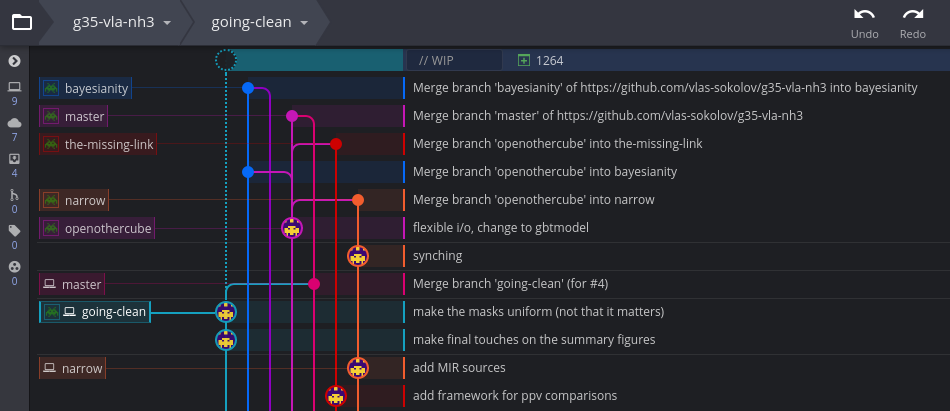
\includegraphics[width=0.7\textwidth]{../Images/ejemplo-ramas.png}
        \caption{origen de la imagen: \url{https://stackoverflow.com/questions/46827112/toggling-branch-tree-view-in-gitkraken}}
    \end{figure}
\end{frame}
\subsection{Main}
\begin{frame}{Main}

    La rama Main (en proyectos antiguos también se puede encontrar como Master) es la rama principal del proyecto y la primera rama que se crea automáticamente al crear el repositorio.

    \begin{itemize}
        \item Rama (normalmente) protegida para evitar código malicioso (de manera intencional o no) sin supervisión.
        \item Generalmente es la rama estable del programa, solo se suben versiones definitivas
    \end{itemize}

\end{frame}
\subsection{Ramas secundarias}
\begin{frame}{Ramas secundarias}
    A estas ramas les daremos nosotros un nombre al crearlas. Son útiles para desarrollar nuevas características del programa o para hacer arreglos de bugs.

    Estas ramas se pueden unir a la principal en cualquier momento del desarrollo para incorporar estos cambios a la rama principal.
\end{frame}
\subsection{Pull request y Merge}
\begin{frame}{Merge}

    Un \textit{Merge} nos permite unificar un conjunto de \textit{commits} en un solo historial.

    Normalmente esto se hace entre los extremos de dos ramas para fusionarlas en una sola.

    Esto puede generar conflictos entre archivos que se pueden resolver con distintos editores de texto o herramientas de gestión de git.

\end{frame}

\begin{frame}{Pull Request}

    Un \textit{pull request} es un mecanismo de GitHub para poder hacer \textit{merge} en proyectos ajenos o para solicitar feedback antes de hacer un merge en tu propio proyecto.

    En ciertos repositorios es obligatorio pasar una \textit{pull request} con varios supervisores para poder contribuir si no eres parte del equipo.

    Tras una \textit{pull request} se hace un merge entre dos ramas.
\end{frame}

\begin{frame}{Fork}

    Un \textit{fork} es un nuevo repositorio que comparte visibilidad y código con un repositorio original.

    Nos permite hacer modificaciones a un código ya existente y después mover esos cambios al repositorio original con una \textit{pull request} (o no).

\end{frame}

\section{Workflows / Actions}
\begin{frame}{Workflows / Actions}

    Github actions es una plataforma de automatización para IC/CD que nos permite crear flujos de trabajo y automatizar pruebas.

    Gratis para repositorios públicos, de pago para repositorios privados (2000\footnote[1]{Minutos de uso en procesos linux, los procesos en Windows cuentan 2x y en MacOs 10x} minutos gratis y 500 MB gratis al mes).


\end{frame}
\subsection{Archivos}
\begin{frame}{Archivos}

    Los archivos para github workflows se guardan en la carpeta \textbf{.github/wokrflows}.

    Estos archivos son de formato \textit{yml}

\end{frame}
\subsection{Estructura básica}
\begin{frame}{Estructura básica}

    Estos archivos siempre tienen que empezar con un nombre para el proceso: \\
    \begin{figure}
        \lstinputlisting[firstline=1, lastline=1, style=customyaml]{../.github/workflows/compile.yml}
    \end{figure}

    Después definimos cuando ejecutar esta acción, puede hacerse en distintas interacciones:
    \begin{figure}
        \lstinputlisting[firstline=2, lastline=2, style=customyaml]{../.github/workflows/compile.yml}
    \end{figure}
\end{frame}

\begin{frame}{Estructura básica}

    Tras los pasos iniciales, empezamos con los ``trabajos''. Los trabajos serán todas las cosas que van a ejecutarse dentro de esta acción.
    Estos trabajos tendrán un nombre expresado como una variable, un entorno de trabajo y una serie de pasos: \\
    \begin{figure}
        \lstinputlisting[firstline=3, lastline=6, style=customyaml]{../.github/workflows/compile.yml}
    \end{figure}
\end{frame}
\begin{frame}{Estructura básica}
    Cada paso tendrá un nombre, un componente que usa para trabajar y posibles variables (dependen del componente):
    \begin{figure}
        \lstinputlisting[firstline=13, lastline=18, style=customyaml]{../.github/workflows/compile.yml}
    \end{figure}
\end{frame}
\subsection{Usos}
\begin{frame}{Usos}

    Estas acciones se pueden usar para automatizar pruebas, hacer versionado de programas, subir archivos o incluso para \href{https://github.com/marcizhu/marcizhu}{jugar al ajedrez}.

    En el \href{https://github.com/marketplace?type=actions}{marketplace} hay miles de acciones ya desarrolladas para hacer casi de todo.

\end{frame}

\section{Repositorios especiales}
\begin{frame}{Repositorios especiales}

    Github se reserva el nombre de ciertos repositorios para crear lo que se denominan ``repositorios especiales''.

    Estos nombres son tu nombre de usuario y tu nombre de usuario seguido de ``.github.io''. El primero crea una descripción que se verá en la portada de tu perfil, el segundo creará una página web principal para tu perfil de github.

\end{frame}
\section{Github Pages}
\begin{frame}{Github pages}

    GitHub pages es un servicio de GitHub que nos permite alojar páginas estáticas bajo el dominio ``github.io''.

    Estas páginas se pueden hacer en cualquier repositorio, posicionarse en distintas ramas y tener dos directorios fuente, la raíz del repositorio o una carpeta ``/docs''

\end{frame}
\begin{frame}

    \begin{figure}[H]
        \centering
        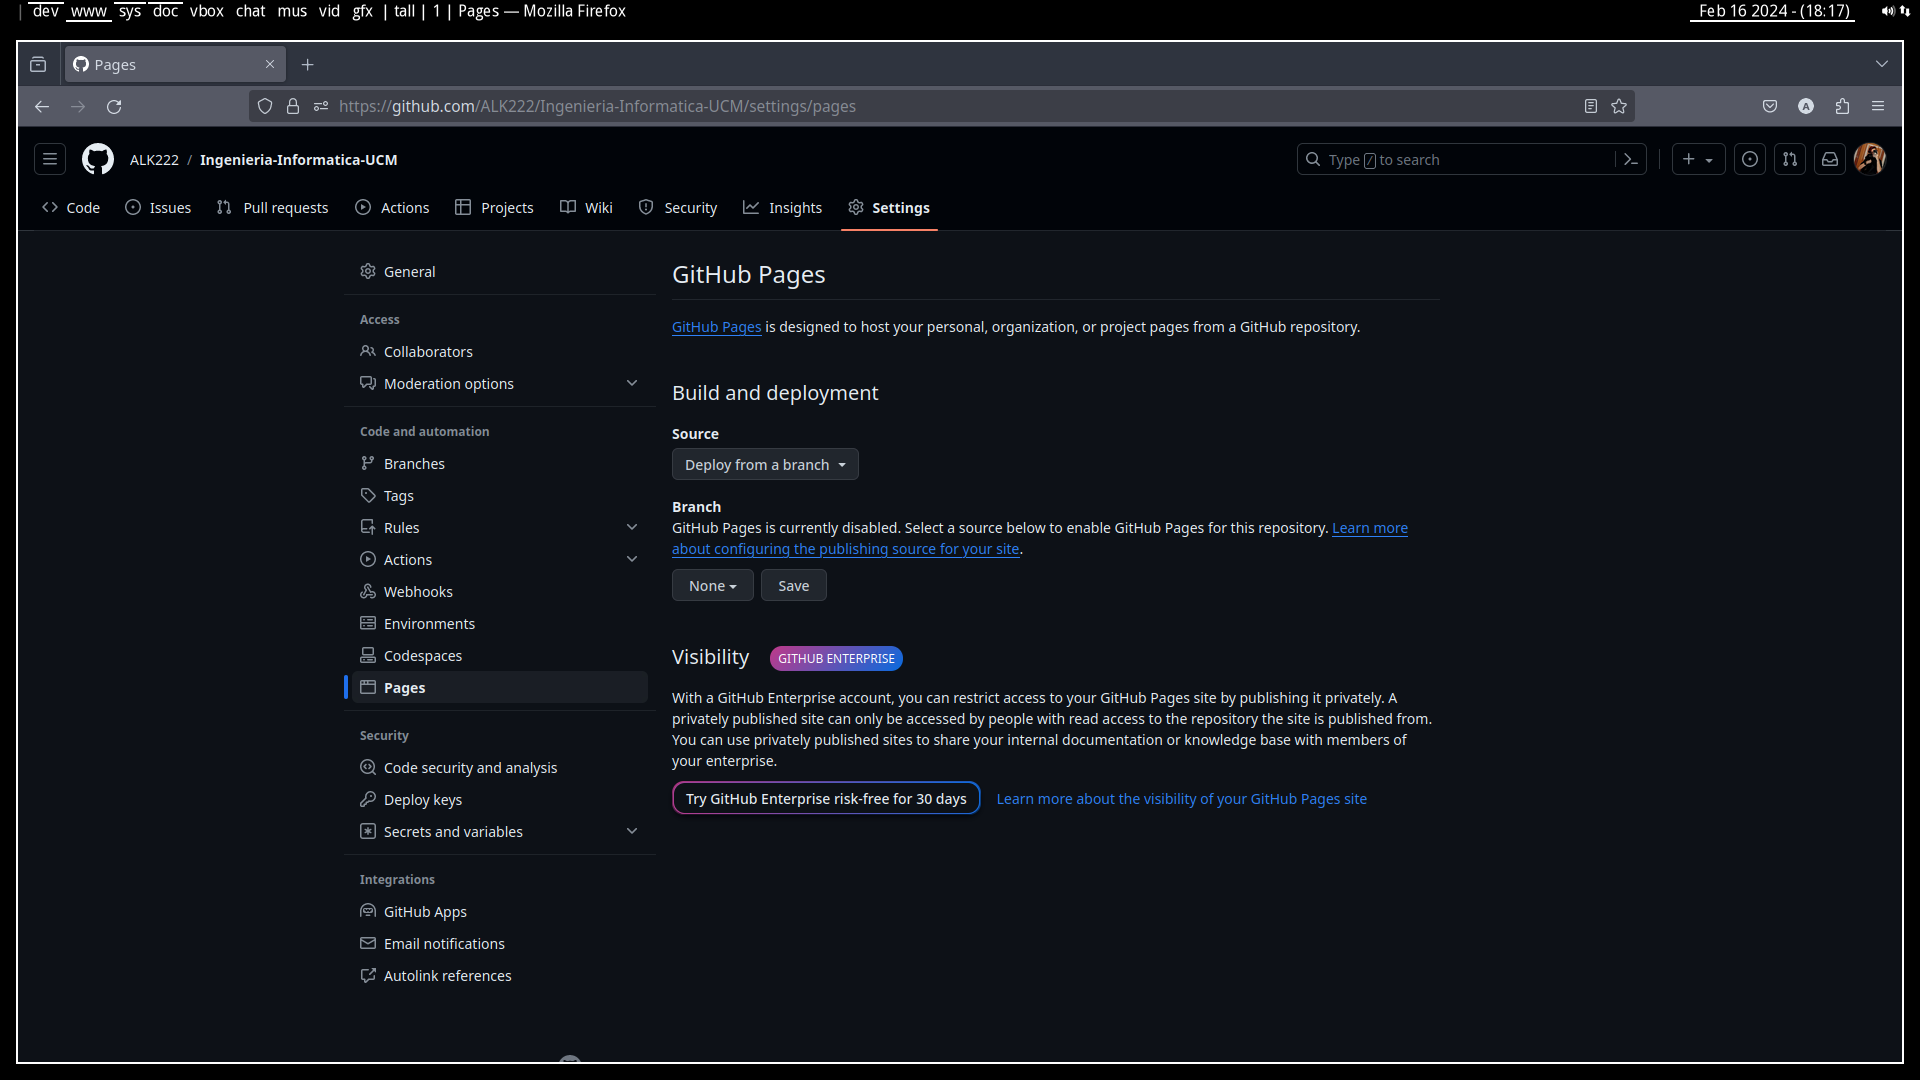
\includegraphics[width=0.7\textwidth]{../Images/github_pages.png}
        \caption{Opciones de GitHub pages antes de publicar la página}
    \end{figure}

\end{frame}

\begin{frame}

    \begin{figure}[H]
        \centering
        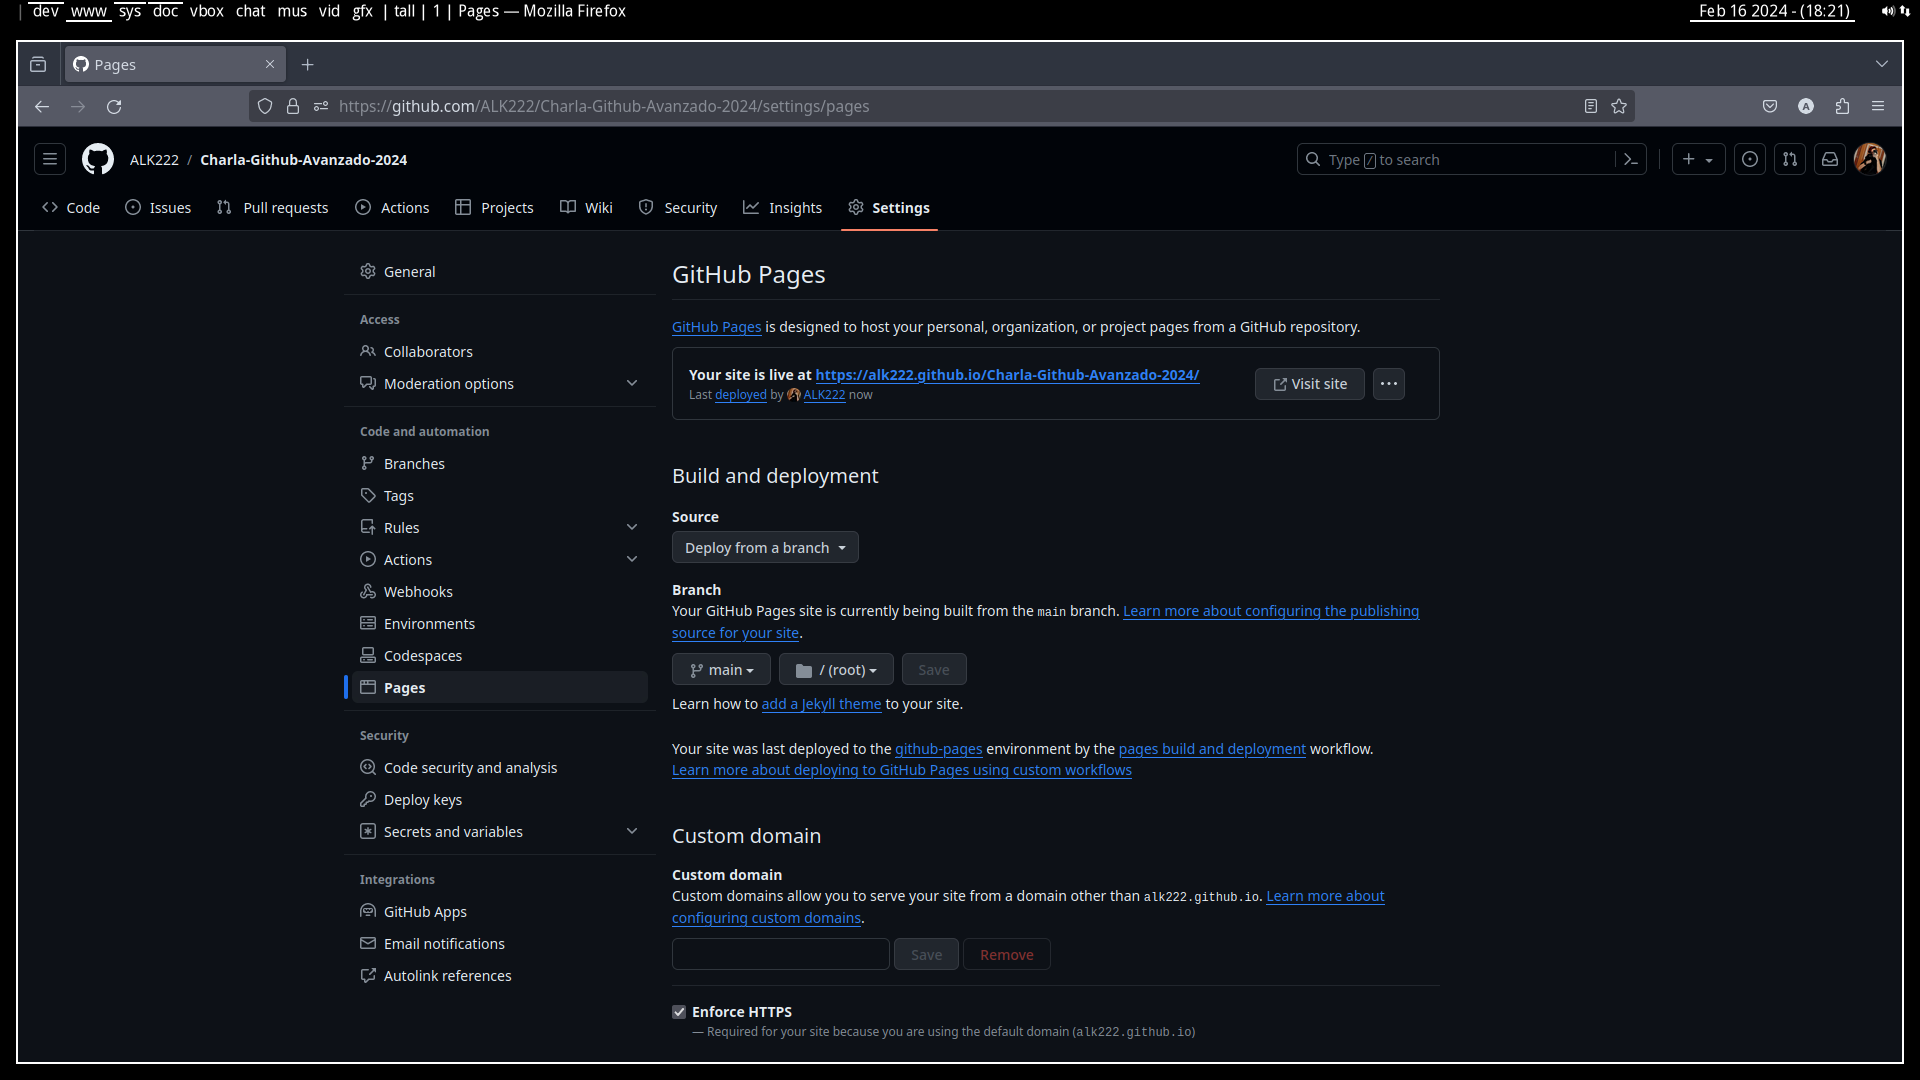
\includegraphics[width=0.7\textwidth]{../Images/github_pages_deploy.png}
        \caption{Opciones de GitHub pages después de publicar la página}
    \end{figure}

\end{frame}
\subsection{Jekyll}

\begin{frame}{Jekyll}

    Estas páginas de github están construidas con Jekyll, permitiéndonos esto hacer pruebas en local, usar HTML o markdown y utilizar todos los plugins disponibles para Jekyll

    \vspace{1cm}
    \begin{columns}
        \column{0.5\textwidth}
        \column{0.5\textwidth}
        \begin{figure}[H]
            \centering
            
\includegraphics[width=0.4\textwidth]{../Images/jekyll.png}

        \end{figure}
    \end{columns}

\end{frame}

\begin{frame}{Fin}

    \begin{tcolorbox}[colback=white,colframe=black!50!white,width=\textwidth,arc=5mm]
        \begin{columns}
            \column{0.4\textwidth}
            \begin{tikzpicture}
                \node [inner sep=0pt] at (0,0) {
\includegraphics[width=4.0cm]{../Images/alk_profile.jpg}};
                \draw [white, rounded corners=\ClipSep, line width=\ClipSep]
                (current bounding box.north west) --
                (current bounding box.north east) --
                (current bounding box.south east) --
                (current bounding box.south west) -- cycle
                ;
            \end{tikzpicture}
            \column{0.5\textwidth}
            \vspace*{10pt} % Adjust vertical spacing as needed
            Alejandro Barrachina \\
            alejba02@ucm.es\\
            github.com/alk222
        \end{columns}
    \end{tcolorbox}

    \begin{figure}
        \centering
        
\includegraphics[width = 0.2\textwidth]{../Images/qr_code.png}
    \end{figure}
\end{frame}
\end{document}